\chapter{TDA Pile/File/Liste}

\textbf{LIFO}: signifie « Last In First Out » Le dernier élément qui a été ajouté est le premier à sortir (Pile).\\
 \\
\textbf{FIFO}: signifie « First In First Out » Le premier élément qui a été ajouté est le premier à sortir (File). \\
\\


\section{Pile}

Une pile (stack) ,de type LIFO , est une liste ou chaque element a acces a l'element suivant en gardant un ordre d'empilage et depilage , on ne peux pas depiler le dernier element sans depiler ceux au sommet de la pile.\\
\\
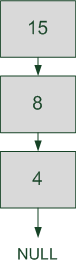
\includegraphics[height=0.35\textwidth,center]{img/pile_c.png}
\\
Une pile peut etre utiliser pour representé un interpreteur par exemple si l'on veux verifier si l'expression est correct cad une parenthese ouvrante = parenthese fermante .\\
[a {g} h i [f] l] ->  expression correct .\\
[a {g} h i [f l] -> expression incorrect .\\



\subsection{Représentation par cellule contigue}

On vas representer notre TDA Pile , qui n'existe a priorie pas en C , par un tableaux avec une variable de controle tel qu'un "sommet" de la pile et de primitive qui vas nous servir a manipuler le tableau .\\
\\
Les primitives de base sur une pile sont : \\
\\
\begin{verbatim}
- void initpile(void);
- void empiler (<type> val); 
- void depiler (<type> *val); 
- int pilevide(void); /*delivre vrais si la pile est vide , faux sinon */
- void sommetpile(<type> *val); /* renvoie la valeur du sommet*/
\end{verbatim}
\\
Le tableaux qui simulera la pile seras declaré en variable globale ainsi que la variable sommet comme ca chaque fonction aura acces a la pile sans a voir a la passé par adressage indirect (par pointeur).\\

\subsubsection{Primitive}

\begin{verbatim}
#define tmax ...
<type> pile[tmax] ;
<type> sommet;

void initpile(void){
  sommet  = -1;
}

void empiler (<type> val){
    if(sommet < tmax-1){
      sommet++;
      pile[sommet]=val;
    }
}

void depiler (<type> *val){
    if(sommet > -1 ){ /*avant d'enlever un element verifier si la pile n'est pas vide*/
      *val = pile[sommet];
      sommet --;
    }
} 

int pilevide(void) {    /*delivre vrais si la pile est vide , faux sinon */
  return (sommet == -1);
}

void sommetpile(<type> *val) { /* renvoie la valeur du sommet*/
    *val=pile[sommet];
}
\end{verbatim}

\subsection{Representation par pointeur}

La variable statique qui represente la pile est un pointeur sur le sommet de la pile .\\
\\
Les primitive de la pile devront etre modifier pour accepter des pointeurs .\\

\subsubsection{Primitive par Pointeur}
\begin{verbatim}
typedef struct element{
  <type> val;
  struct element *suivant;
} t_element;

t_element * pile;

void initpile(void){
  pile=NULL;
}

int pilevide(void){
  return(pile==NULL);
}

void empiler(<type> val){
  t_element *nouv=malloc(sizeof(t_element));

  nouv->val=val;
  nouv->suivant=pile;
  pile=nouv;
}

void depiler(<type> *val){
  t_element * sommet ;
  if(!pilevide()){    /*avant d'enlever un element verifier si la pile n'est pas vide*/
      *val=pile->val;  
      pile=sommet->suivant;
      free(sommet);
  }
}

void sommetpile(<type> *val){
  if(pile!=NULL){
    *val=pile->val;
  }
}
\end{verbatim}


\section{File}

Une file, de type FIFO , est une liste chainée ou chaque element a acces a l'element suivant en gardant les contraintes d'une liste ,on ne peux pas acceder directement au n-element de la liste sans la parcourire.\\
\\
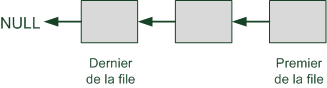
\includegraphics[width=0.5\textwidth,center]{img/file_c.png}
\\

\subsection{Representation contigue}

Meme principe que pour la pile sauf que l'ajout ou le retrait d'élément peux se faire soit du debut soit de la fin .\\
Necessite la declaration de variable de controle globale \textbf{tete},\textbf{queue} et du nombre d'element présent dans la file .\\
Un probleme ce pose quand on utilise cette representation c'est que lors de la suppression d'une valeur en tete de file , la case supprimé restera libre or les element qui seront derriere la tete ne seront pas utilisé , il reste donc de l'espace libre dans le tableau mais inaccessible . Pour cela nous allons utilise une file circulaire .\\

Les primitives de base seront plus au moins les meme que celle de la pile : \\
\\
\begin{verbatim}
- void initfile(void);
- void ajouter (<type> val); /*ajout en queue de la file */
- void retirer (<type> *val); /*retrait en tete de file */
- int filevide(void);
- int filepleine(void);
\end{verbatim}

\subsubsection{Primitive}
\begin{verbatim}
#define tmax ....
<type> file[tmax];
<type> tete,queue,nb_val;

void initfile(void){
  tete=0;
  queue=tmax-1;
  nb_val=0;  
}

void ajouter (<type> val){  /*ajout en queue de la file */
    if(nb_valeur < tmax){
        if(queue == tmax-1){
          queue=0;
        }
        else{
          queue++;
        }
      file[queue]=val;
      nb_val++;
    }
}

void retirer (<type> *val){ /*retrait en tete de file */
  if(nb_val > 0){
    *val=file[tete];
    nb_vall--;

    if(tete==tmax-1){
      tete=0;
    }
    else{
      tete++;
    }
  }
}

int filevide(void){
  return(nb_val==0);
}

int filepleine(void){
  return(nb_val==tmax);  
}
\end{verbatim}

\section{Liste}

Les piles et files sont des liste chainée mais avec des accés aux elements plus particulier. Une liste chainée peux acceder aux elements de ces voisins grace a des pointeurs.\\


%%%%%%%%%%%%%%%%%%%%%%%%%%%%%%%%%%%%%%%%%%%%%%%%%%%%%%%%%%%%%%%%%%%%%%%%%%%%%%%%%%%%%%%%%%%%%%%%%%

\end{document}